\section{CORBA}\label{capitolo3}
L'acronimo \textbf{CORBA} significa \emph{Common Object Request Broker Architeture} ed è il cuore dell'\emph{Open Managment Architeture} (OMA) un prodotto sviluppato dall'\emph{Open Managment Group} (OMG).\\
L'OMA è definito come un \emph{open framework} per applicazioni Object-Oriented distribuite, esso aiuta l'interoperabilità e fornisce mappature per diversi linguaggi di programmazione. Questo framework permette la progettazione di applicazioni distribuite come un insieme di oggetti cooperanti. I diversi programmi interagiscono tra loro come fossero eseguiti su di una singola macchina, trascurando il linguaggio con i quali sono stati sviluppati e l'hardware sui quali sono eseguiti.\\
L'OMG è un organismo di standardizzazione, esso fornisce solamente le specifiche e non l'implementazione di CORBA.\\
L'OMA definisce un \emph{Interface Definition Language} per specificare le API degli oggetti CORBA in termini di interfacce ed operazione. Un esempio della struttura di un sistema CORBA è mostrato in \figurename"\ref{fig:orb}.
\begin{figure}
\centering
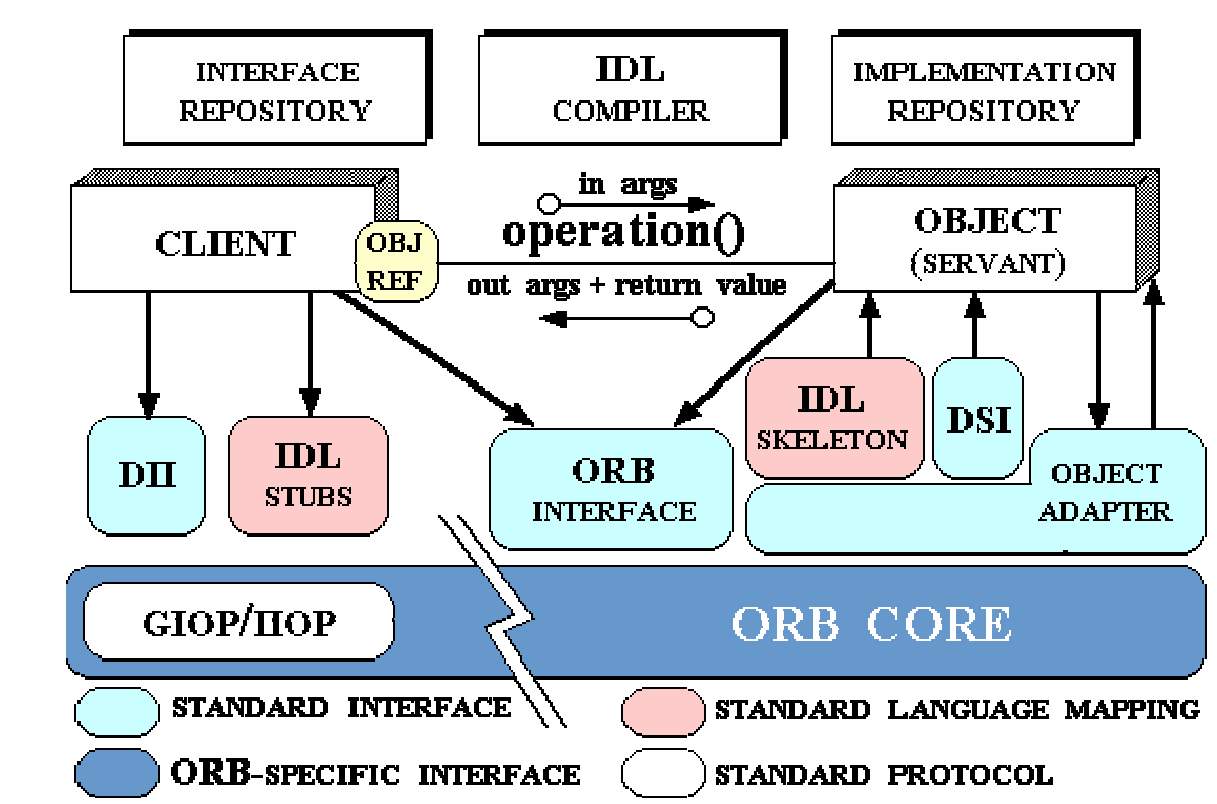
\includegraphics[width=0.7\linewidth]{img/orb}
\caption{Struttura di un sistema CORBA}
\label{fig:orb}
\end{figure}
L'\emph{Object Request Broker} è composto da diversi componenti, i principali sono il \emph{client}, il \emph{servant} e l'\emph{ORB Core}:
\begin{description}
	\item[Client:] è il componente che invoca i diversi servizi, esso mantiene un riferimento agli oggetti remoti.
	\item[Servant:] questo componente \emph{rappresenta} un oggetto CORBA, esso non è un vero e proprio oggetto in quanto gli oggetti CORBA sono solamente un concetto mentre un \emph{servant} è un oggetto nel linguaggio target che viene utilizzato per implementare uno o più oggetti CORBA. Quando un processo server riparte esso crea un nuovo \emph{servant} per rappresentare lo stesso oggetto CORBA.
	\item[ORB Core:] è responsabile dello smistamento e dell'inoltro delle chiamate agli oggetti remoti nascondendo così la comunicazione al programmatore. Il suo compito è quello di localizzare gli oggetti remoti, comunicare le richieste a questi oggetti, attendere un risultato ed infine restituire il risultato a chi lo ha richiesto.
	\item[ORB Interface:] è l'interfaccia standard per accedere ad un servizio del core, questo disaccoppia client e server da una specifica implementazione dell'ORB.
	\item[IDL Stub e Skeleton:] costruito dalle interfacce degli oggerri remoti tramite il compilatore IDL, insieme all'ORB permette il dispacciamento delle richieste al giusto oggetto remoto.
	\item[Dynamic Invokation Interface:] (DII) interfaccia standard utilizzata dal client per accedere ai servizi forniti da un oggetto remoto la cui interfaccia non era conosciuta a tempo di compilazione.
	\item[Dynamic Skeleton Interface:] (DSI) interfaccia standard utilizzata per implementare un oggetto remoto.
	\item[Object Adapter:] è il componente che gestisce la comunicazione tra l'oggetto remoto e l'ORB, esso incorpora i meccanismi e le policies principali per implementare le seguenti operazioni:
	\begin{itemize}
		\item Registrare, attivare e disattivare i servant
		\item Creare e interpretare i riferimenti agli oggetti
		\item mediare l'invocazione dei servizi
	\end{itemize}
	\item[GIOP e IIOP:] sono i protocolli utilizzati per connettere il client e il server sono standardizzati dal OMG.
\end{description}
Il \emph{Portable Object Adapter} (POA) come abbiamo visto, è un componente situato tra l'ORB e i servant, il client effettua una richiesta utilizzando un riferimento all'oggetto remoto, la richiesta viene ricevuta dall'ORB che inoltra la richiesta al POA che ospita l'oggetto. Il POA dispaccia la richiesta al servant di competenza il quale esegue l'operazione e restituisce il risultato al POA che a sua volta la inoltra all'ORB che la restituisce al client. Il POA deve soddisfare tre requisiti:
\begin{itemize}
	\item creare riferimenti agli oggetti per permettere al client di raggiungere l'oggetto remoto.
	\item assicurarsi che ogni oggetto target sia riferito ad un servant.
	\item ricevere le richieste dal parte client dell'ORB e indirizzarle verso il servant adatto.
\end{itemize}
Oltre alla parte principale di CORBA esistono una serie di servizi che forniscono una serie di funzionalità a supporto dell'integrazione e dell'interoperabilità degli oggetti distribuiti. Questi oggetti sono chiamati \emph{CORBA SErvice} o \emph{Object Service} e sono definiti come standard in CORBA da interfacce specificate in IDL. I principali servizi sono il servizio di \emph{Naming} e di \emph{Trading Object} che permettono al server di esporre i suoi servant. I servizi \emph{Event} e \emph{Notification} supportano la comunicazione asincrona multipla, il servizio \emph{Transaction} fornisce un supporta ai sistemi transazionali.\\
Il sistema CORBA, infine, fornisce delle \emph{horizontal facilities} e delle \emph{vertical facilities}, le prime si posizionano tra il middleware CORBA e i potenziali servizi utilizzati nel dominio di applicazione come una \emph{printing facility} o una \emph{mobile agent facility}.
Le \emph{Vertical Facilities} definiscono delle interfacce standard per quegli oggetti che ogni settore del dominio vuole condividere.
\subsection{CORBA e Java}
Java include di default un'implementazione base, ma completamente funzionante di CORBA, un IDL per il compilatore Java e un Naming Service.\\
Lo scopo dell'IDL è quello di permettere la definizione delle interfacce degli oggetti in un modo indipendente dal linguaggio di programmazione utilizzato per l'implementazione. Per chiamare una funzione di un oggetto CORBA tutto quello che è necessario al client è l'IDL dell'oggetto. l'IDL supporta \emph{multiple inheritance} e \emph{genericity}, esso supporta parametri sia in input che in output sia bidirezionali, le operazioni possono sollevare delle \emph{eccezioni} definite nell'IDL, infine, esso fornisce una serie di tipi di dato come \texttt{string, boolean, int, long, float} e \texttt{double} ma permette anche la definizione di tipi complessi tramite \texttt{struct, sequence, array, typedef, enum} e \texttt{union}.
Un esempio di file IDL è quello del Listato \ref{lst:idlexemp}
\lstinputlisting[language=IDL,caption="Esempio di file IDL",label=lst:idlexemp]{listati/account.idl}
Per un'analisi approfondita sullo sviluppo di una applicazione con CORBA si rimanda a \cite{cugola:corba} e \cite{sun:corba}